In this section we do some further analysis on the data gathered from LJ. 

\subsubsection{Do attractive people group together?}\label{sec:att_dist}

In order to better understand attractive members, we studied how they are distributed in the community. Are they distributed uniformly or follow some patterns.  Specifically,  for each community $\Cc$, we computed the percentage of attractive friends of all members $v\in\Cc$, i.e., for each member $v$, we computed
\[
\frac{\sum\limits_{v'\in\partial v \cap \Cc } a_{v'}}{\partial v \cap \Cc }.
\]  
For each community, we divide these numbers into two separate sets for attractive and unattractive people, and computed the average of each set. The box plot in Fig. \ref{fig: perc att} summarizes the statistics of these averages computed for the communities under study. There is a clear difference between the percentage of attractive friends of attractive and unattractive people. Attractive people seem to have a much higher percentage of attractive friends. 


\subsubsection{Do social people group together?}

Similar to Section \ref{sec:att_dist}, we can study the distribution of social people in a community. For each person we compute the percentage of its friends that are social. Again we divide these numbers into two sets which corresponds to social and asocial people. Fig.~\ref{fig: perc social} summarizes the distribution of each set. It demonstrates significant distinction between the two distributions.  According to the plot, on average about $60\%$ of a social person's friends are social themselves, while this percentage is less that $20\%$ for an asocial person.

\begin{figure}
\begin{center}
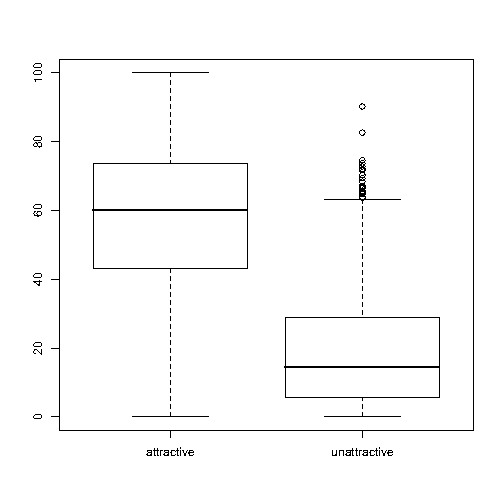
\includegraphics[width=80mm]{Rplot.pdf}\caption{Percentage of attractive friends of attractive/unattractive members}\label{fig: perc att}
\end{center}
\end{figure}

\begin{figure}
\begin{center}
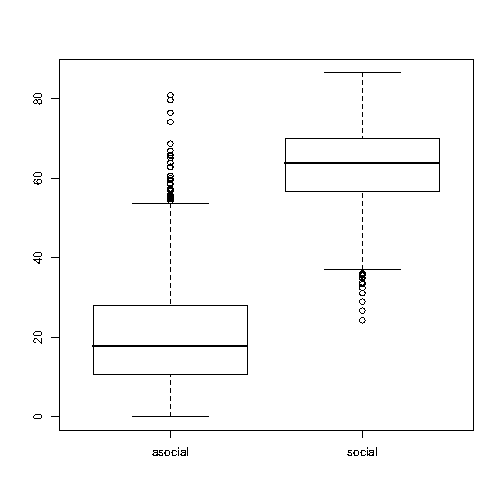
\includegraphics[width=80mm]{Rplot_soc.pdf}\caption{Percentage of social friends of social/asocial members}\label{fig: perc social}
\end{center}
\end{figure}


\subsubsection{Puzzle}

Several studies point to the fact that the growth of a community is highly dependent on its clustering coefficient.
This coefficient is defined as the ratio of closed to open triads in the friendship subgraph
induced by the members of a community.

\begin{figure}
  \begin{center}
    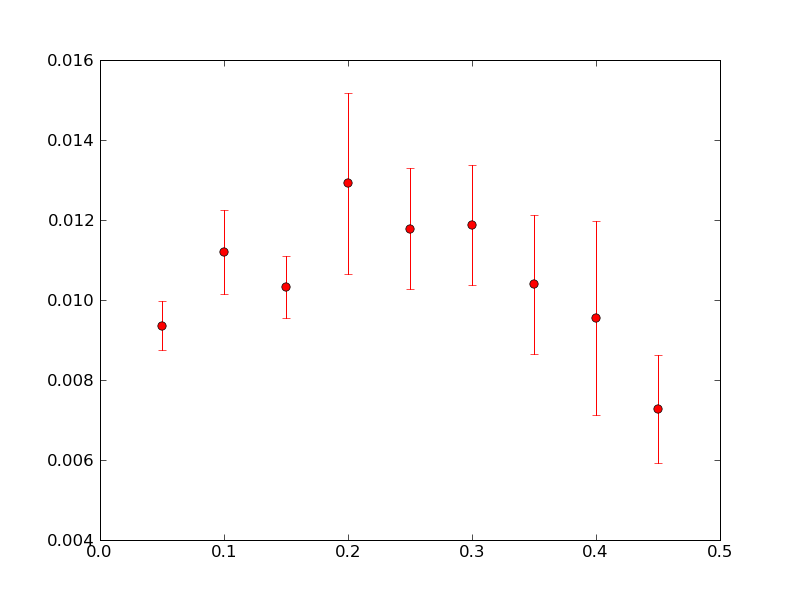
\includegraphics[width=8cm]{first.png}
    \caption{Community growth rates vs. ratio of closed to open triads: $1^{\rm st}$ snapshot}\label{fig:edge-a}
    \end{center}
\end{figure}


In Backstrom et al. paper \cite{group_formation}, the authors observe that if a community is highly connected, then it is less probable to grow.  This result is in contrast to the empirical evidence \cite{group_formation}  that suggests that a person is more probable to join a community,  if his/her friends inside the community are more interconnected.


\begin{figure}
  \begin{center}
    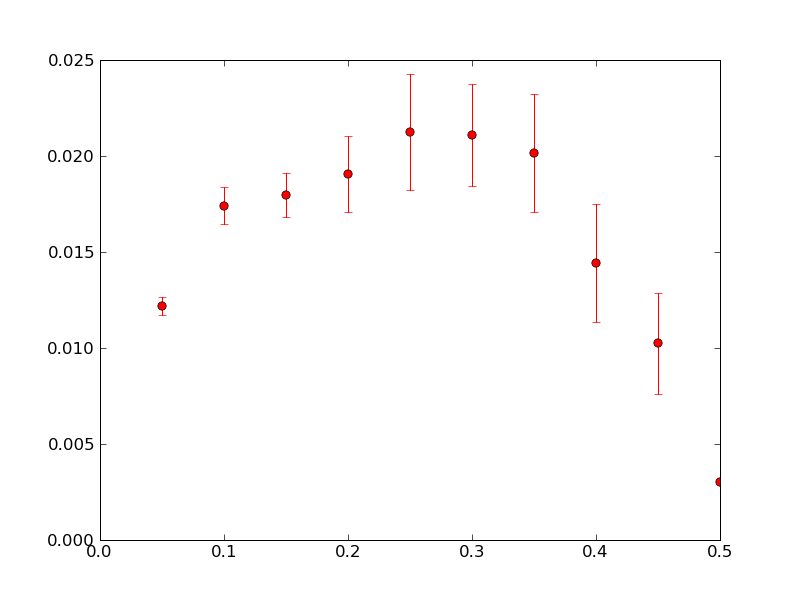
\includegraphics[width=8cm]{second.png}
    \caption{Community growth rates vs. ratio of closed to open triads: $2^{\rm nd}$ snapshot}\label{fig:edge-b}
    \end{center}
\end{figure}


In Figures \ref{fig:edge-a}-\ref{fig:edge-f}, for each snapshot, we plot the communities growth rates  as a function of their clustering coefficient.  Communities are binned together with respect to clustering coefficient. The growth rate is  decreasing for the communities that have clustering coefficients  higher than $0.3$, especially for the first two snapshots.  On the other hand, the number of communities  with large clustering coefficient  is much smaller than the ones with small clustering coefficient.

\begin{figure}
  \begin{center}
    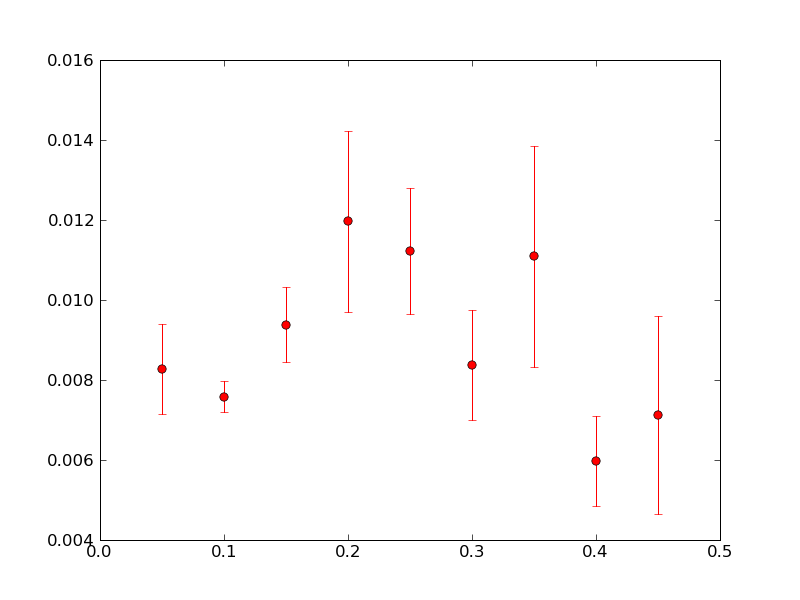
\includegraphics[width=8cm]{third.png}\label{fig:edge-c}
    \caption{Community growth rates vs. ratio of closed to open triads: $3^{\rm rd}$ snapshot}
    \end{center}
\end{figure}




In order to understand the relationship between  the clustering coefficient and the growth of a community, we divided 
the communities into two groups: $\mathcal{C}_h$ and $\mathcal{C}_l$, i.e., those that have  a clustering coefficient higher than the average, and those that have a  clustering coefficient less than the average. 

\begin{figure}
  \begin{center}
    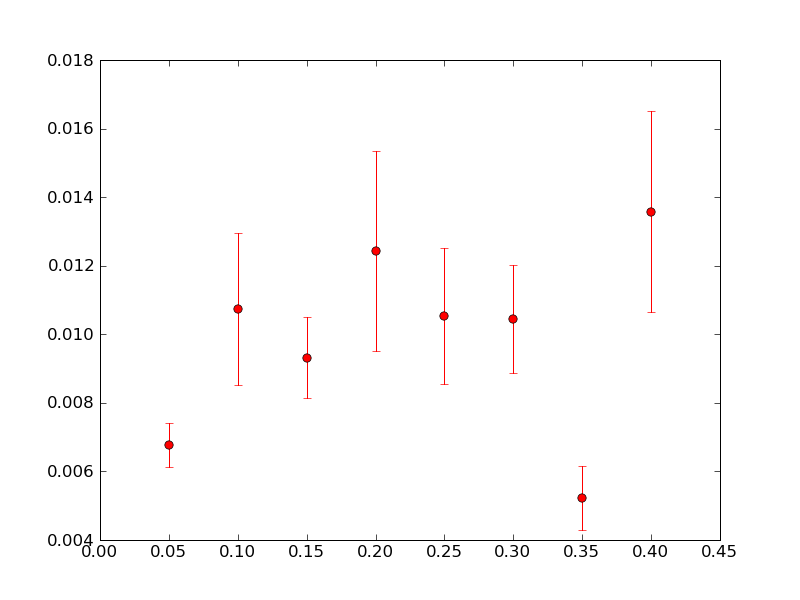
\includegraphics[width=8cm]{fourth.png}\label{fig:edge-d}
    \caption{Community growth rates vs. ratio of closed to open triads: $4^{\rm th}$ snapshot}
    \end{center}
\end{figure}




For each community $\Cc$, we computed the percentage of people in the fringe that only have one friends inside the community, i.e., 
\[
\frac{|\{x\in\mathcal{F} : \; x \textmd{ has only one friend in } \mathcal{C} \}|}{|\mathcal{F}|},
\]
and took the average among $\mathcal{C}_l$ and $\mathcal{C}_h$ separately. 
We found that for communities in $\mathcal{C}_l$ the average of this ratio is $86.6\%$, while for $\mathcal{C}_h$ it is
$76.9\%$.
Thus in the fringe of highly connected communities, on average, there are fewer people that have only one friend inside the community. Then we computed the probability 
of joining a community from its fringe for those who have only one friend inside. We took the average over $\mathcal{C}_l$ and $\mathcal{C}_h$ separately. 
The average probability of joining for such users among $\mathcal{C}_h$ communities turned out to be $8.4\times10^{-5}$, while the average of the same 
quantity for communities in $\mathcal{C}_l$ was $15.8\times 10^{-5}$ which is about two times  more. Therefore, since the majority of fringe consists of those who have only one friend inside, this partly describes the dichotomy. In other words the growth behavior  of a community is mainly determined by those in the fringe that have only one friend inside, because they are the majority of the fringe members; On the other hand, our empirical results suggest that these people are less probable to join a community if its is highly connected. 

\begin{figure}
  \begin{center}
    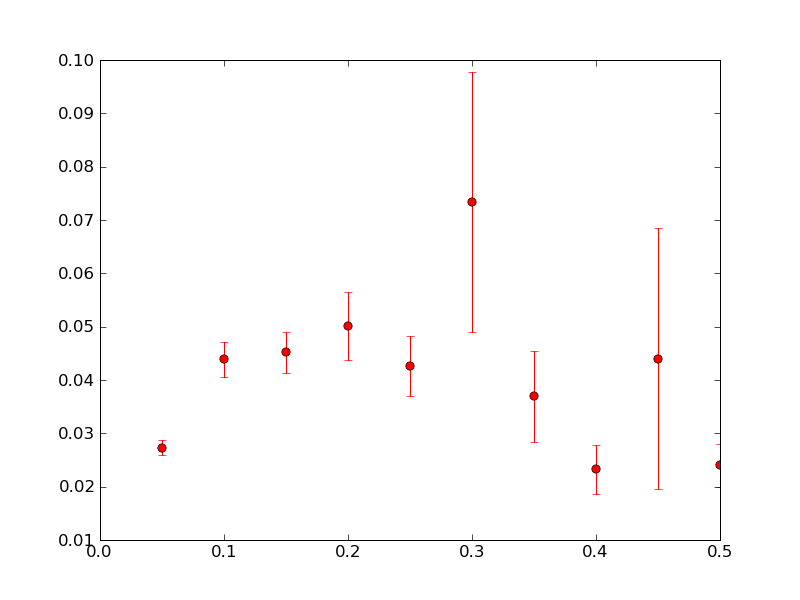
\includegraphics[width=8cm]{fifth.png}\label{fig:edge-e}
    \caption{Community growth rates vs. ratio of closed to open triads: $5^{\rm th}$ snapshot}
    \end{center}
\end{figure}


\begin{figure}
  \begin{center}
    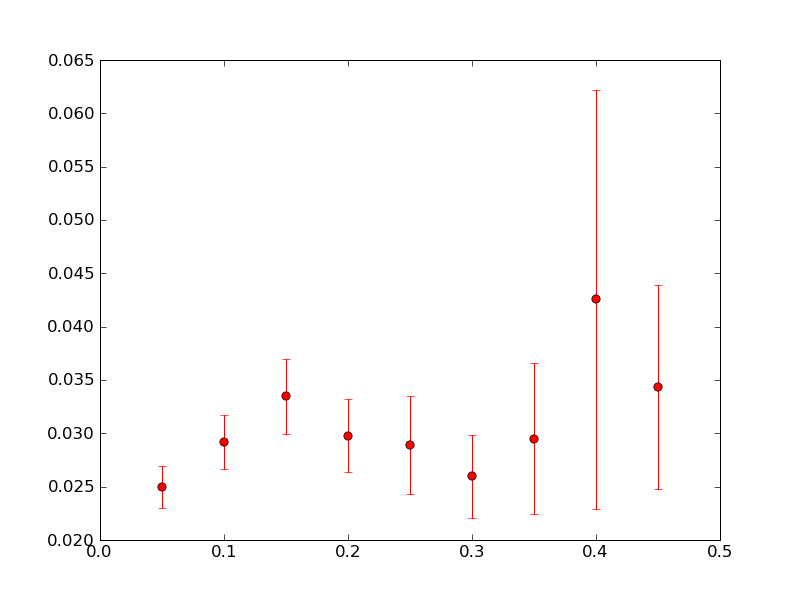
\includegraphics[width=8cm]{sixth.png}
    \caption{Community growth rates vs. ratio of closed to open triads: $6^{\rm th}$ snapshot}\label{fig:edge-f}
    \end{center}
\end{figure}



%\newpage
%\subsection{Simulation}
%
%In this section we propose a simple model for simulating the evolution of communities through time. First we observe the evolution of a community during some initial time period, and label its members as attractive and unattractive. Then to each member of the fringe we assign a probability $p_j$, the probability of joining the community, as follows
%\[
%p_{j} = \frac{1+C_{\rm a}N_a+C_{\rm una}N_{\rm una}}{1+C_0+C_{\rm a}N_a+C_{\rm una}N_{\rm una}},
%\]
%where $N_a$ is number of attractive friends of this member inside the community, and $N_{\rm una}$ is its number of unattractive friends. Also $C_0$, $C_{\rm at}$, and $C_{\rm una}$ are constants. In our simulations, after trying to find the parameters that fit the data, we used $C_0 = 250$, $C_{\rm a} = 2$, and $C_{\rm una}=1$, which seemed to give the best results. Although the model can predict all the
%non-growing communities correctly, it could predict only about half of the growing communities as growing. We would like to try different models in order to predict the growth.
%
\subsection{Further study of attractive people}
Let us focus on our measure \emph{attractivity} to understand more about what it really represents in the community
and its effects on growth.

\begin{itemize}
\item Are recent members of the community mostly attractive?
\end{itemize}

In Table \ref{table:rec}, for each snapshot,  we show what percentage of the people who
have joined the community in the previous snapshot are attractive.
 Especially for the first three snapshots, where
time between the snapshots are about a week, almost half of the recent members of the community are 
attractive. Given the fact that the attractive members in a community are much less than the unattractive 
ones, the recent members are more likely to be attractive.

\begin{table}[htdp]
\caption{Average percentage of attractive people among the people who have just joined}
\begin{center}
\begin{tabular}{|c|c|c|c|c|c}
\hline
snapshot & 2 & 3 & 4 & 5 \\ \hline
average percentage of   & 0.524 & 0.510 & 0.550 & 0.382 \\
attractive people  &  &  & &  \\ \hline
\end{tabular}
\end{center}
\label{table:rec}
\end{table}

%\begin{figure}
%\begin{center}
%\includegraphics[width=120mm]{rec_att.pdf}\caption{Distribution of attractivity of new comers}\label%{fig:rec_att}
%\end{center}
%\end{figure}

\begin{itemize}
\item Are there people who are always attractive?
\end{itemize}

Among the first four snapshots, for each person in a community, we computed the number of snapshots
he/she has been attractive. Table  \ref{table:all} shows the number of people that were attractive in just one snapshot, two snapshots etc.
So, we can conclude that the most people don't stay attractive for a long time.

\begin{table}[htdp]
\caption{Frequency of being  attractive for difference people}
\begin{center}
\begin{tabular}{|c|c|c|c|c|}
\hline
number of snapshots & 1 & 2 & 3 & 4  \\ \hline
number of people  & 29,255 & 6,171 & 3,954 & 34 \\ \hline
\end{tabular}
\end{center}
\label{table:all}
\end{table}%

\begin{itemize}
\item Is attractiveness of a person group-dependent?
\end{itemize}

One question to ask is whether knowing that a person is considered active in a group increases the chance of $v$ being attractive in other groups that contain $v$ as well. Similarly, does being unattractive in one community makes it more probable to be unattractive in other groups too. Let a person $v\in\Vc$ belong to $n_v$ different communities, $\mathcal{C}_1,\ldots,\mathcal{C}_{n_v}$. The vector  $(a_v(\Cc_1),\ldots,a_v(\Cc_{n_v})$ represents attractiveness of $v$ in these communities. For each person $v\in\Vc$ define 
\begin{align}
p_v\triangleq\max\left(\frac{\sum\limits_{i=1}^{n_v} a_v(\Cc_i)}{n_v},1-\frac{\sum\limits_{i=1}^{n_v} a_v(\Cc_i)}{n_v}\right).
\end{align}
If $v$ belongs to 5 communities and its attractiveness status vector is $(0,1,1,0,1)$  or $(1,0,0,1,0)$ in both cases $p_v=60\%$. From our data, we looked at  $\frac{1}{n}\sum_i p_i  $. Table \ref{table:glob} shows strong correlation among the variables.

\begin{table}[htdp]
\caption{Attractivity of a user in different communities}
\begin{center}
\begin{tabular}{|c|c|c|c|c|}\hline
snapshot & 1 & 2 & 3 & 4  \\ \hline
ratio  & 0.916 & 0.925 & 0.989 & 0.89 \\ \hline
\end{tabular}
\end{center}
\label{table:glob}
\end{table}%



